\documentclass[12pt]{article}

\usepackage{amsmath,amsthm,amssymb}
\usepackage{graphicx}

\newtheorem{thm}{Theorem}
\newtheorem{lem}[thm]{Lemma}
\newtheorem{cor}[thm]{Corollary}
\newtheorem{prop}[thm]{Proposition}
\newtheorem{defn}[thm]{Definition}
\newtheorem{ex}[thm]{Example}
\newtheorem{prob}[thm]{Problem}
\newtheorem{alg}[thm]{Algorithm}
\newtheorem{nota}[thm]{Notation}
\newcommand{\N}{\mathbb{N}}
\newcommand{\Z}{\mathbb{Z}}
\newcommand{\Q}{\mathbb{Q}}
\newcommand{\R}{\mathbb{R}}


\begin{document}

\centerline{\large {\bf Chaos in Seemingly Simple Optical Systems} $_{Liam Packer}$}

\section*{Abstract}

A particularly illuminating application of analysis in dynamical systems is to that of
(nonlinear) optical systems. These systems are characterized by a nonlinear response of a
material by an incident electromagnetic wave, allowing for the existence of a variety of
phenomena such as laser pumping, frequency-doubling, four-wave-mixing, and many more
\cite{shen_principles_1984}. What is less well known is that chaotic behavior can emerge in
even the simplest of these systems. Both in optical pumping and nonlinear wave propagation,
it was predicted that chaotic behavior was possible and emergent when a particular set of
conditions are met depending on the system. As an example, in the simple case of optical
pumping of a nonlinear gain material, the system can be modeled by a set of equations known
as the Maxwell-Bloch equations \cite{harrison_chaos_1986} which bear striking similarity to
the Lorenz system (and in fact, reduce to the Lorenz system under certain conditions on the
parameters). We'll be analyzing a different, but still seemingly simple, optical system
known as a ring cavity dielectric medium. We will be following
\cite{ikeda_multiple-valued_1979} and \cite{ikeda_optical_1980} closely. It has been shown
\cite{ikeda_multiple-valued_1979} that under reasonable boundary conditions on the ring, the
dynamics of the system are given by

\begin{align*}
  E(t) &= A + BE(t - t_R) \exp\{i[\phi(t) - \phi_0]\},\\
  \gamma^{-1}\dot{\phi}(t) &= -\phi(t) + \text{sgn}(n_2)|E(t - t_R)|^2
\end{align*}
where $\gamma$ is a relaxation rate parameter, $A$ is proportional to the amplitude of the
incident field, $B$ characterizes the dissipation of the electric field through the cavity,
and $t_R$ a time delay. The stationary solutions $E_s$ satisfy
\[[1 + B^2 - 2B\cos(|E_s^2 - \phi_0)]|E_s|^2 = A^2\]

Variation of the parameters $A$, $B$, $\phi_0$ will yield different possible steady-state
solutions. As the steady-state solution $E_s$ becomes unstable through the variation in
parameters, the system undergoes a sequence of bifurcations eventually yielding a chaotic
regime with an associated strange attractor \cite{ikeda_optical_1980}. The analysis of the
system can be done by introducing a difference equation which illuminates the
period-doubling sequence followed by chaotic regimes \cite{harrison_chaos_1986}.

\section*{A Brief Introduction to Nonlinear Optics}
\subsection*{Nonlinear Polarization}
First, we will get at taste of how higher-order dependence of a dielectric medium on an
electric field can produce interesting effects, especially the effect of an
intensity-dependent index of refraction. This will be key in the model we will study, for
this non-linear response of the medium in the presence of an electric field will pave the
way for a road to chaos.

In typical optics, we consider a dielectric material which has a \textit{linear}
relationship with incident electromagnetic waves. For simplicity, we consider only the
electric field. We say that a material is \textit{polarized} when, in a classical
approximation, an electric field aligns the molecular dipoles of the material in a certain
direction. The direction of polarization is in general dependent on the shape of material,
type of material, position in the material, and the frequency and strength of the incident
electric field. In the simplest model, we assume that the reaction of the material's
molecular dipole moment density $\mathbf{P}$ is \textit{linear} in the electric field
strength, $\mathbf{P} \propto \mathbf{E}$, where $\mathbf{P}\equiv$ ``average dipole
moment'' for a very small region of space. In a first course of electromagnetics, the
proportionality is taken to be direct, so that $\mathbf{P} = \epsilon_0\chi_e \mathbf{E}$,
where $\chi_e$ is known as the ``electric susceptibility'' of the medium \cite{TODO
  GRIFFITHS} and quantifies how strong the reaction of the molecules in the material is to
the incident electric field. In general, the relationship can be true up to a linear
transformation, so that $\mathbf{P} = \epsilon_0\chi^{(1)}(\mathbf{E})$, where $\chi^{(1)}$
is known as the first-order (or linear) susceptibility, a linear map defined at each point
in the dielectric medium \cite{TODO GRIFFITHS}. This first-order tensor allows for the
medium to prefer certain polarization directions at different locations, although the
relationship is still linear and involves only first ``powers'' of $\mathbf{E}$. This linear
relationship means that the resulting \textit{intensity} of the total electric field in the
medium can only be linear in the incident electric field.

Next, we introduce nonlinearities in the dependence of the polarization $\mathbf{P}$ on the
electric field $\mathbf{E}$ by expanding $\mathbf{P}$ as a power-series in higher-order
susceptibility tensors \cite{TODO BOYD}:

\begin{align*}
  \mathbf{P}(t) &= \epsilon_0[\chi^{(1)}(\mathbf{E}(t)) + \chi^{(2)}(\mathbf{E}, \mathbf{E}) +
                  \chi^{(3)}(\mathbf{E}, \mathbf{E}, \mathbf{E}) + \cdots]\\
                &= \mathbf{P}^{(1)}(t) + \mathbf{P}^{(2)}(t) + \mathbf{P}^{(3)}(t) + \cdots,
\end{align*}
where we define the $n^{th}$ order polarization to be
$\mathbf{P}^{(n)} = \chi^{(n)}(\mathbf{E}, \cdots, \mathbf{E})$. In more typical component
notation, the $n^{th}$ order polarization component $P^i$ can be written as
$P^i = \sum_{j,k,\cdots}\chi^{(n)}_{ij\cdots}E^jE^k\cdots$. We can immediately see the
nonlinear dependence of $\mathbf{P}$ on $\mathbf{E}$ through the products of components $E^j$
proportioned by $\chi_{ij\cdots}$. We note that the polarization $\mathbf{P}(t)$, in this
approximation, only depends on the electric field at the \textit{current time $t$},
$\mathbf{E}(t)$. Physically this means the medium responds instantaneously to the electric
field, which we'll assume from here on out. In general the dependence is non-instantaneous
in the case of materials with dispersion or loss \cite{TODO BOYD}.

\subsection*{Intensity-Dependent Refractive Index}
For simplicity, we drop the tensors and consider the polarization magnitude and electric
field magnitude. The third-order polarization magnitude $P^{(3)}(t)$ is then expressed as
$P^{(3)}(t) = \epsilon_0\chi^{(3)}E^3(t)\propto E^3(t)$, where $\chi^{(3)}$ is now a
\textit{scalar}, meaning $P$ is linearly dependent on the cube of $E$. If we assume a
monochromatic wave, $E(t) = \mathcal{E} \cos \omega t$, then using the identity $\cos^3\omega
t = \frac14 \cos(3\omega t) + \frac34 \cos \omega t$:
\[ P^{(3)}(t) = \frac14 \epsilon_0\chi^{(3)}\mathcal{E}^3 \cos 3\omega t + \frac34
  \epsilon_0\chi^{(3)}\mathcal{E}^3\cos\omega t.\]


%% TODO rework this paragraph to just get right to the point
We can see that two frequency terms emerge: a component with frequency $3\omega$, known as
the third-harmonic generated component, and a component with the original frequency $\omega$
which gives rise to an intensity-dependent index of refraction. This intensity-dependent
effect is exactly what we needed. Writing the index of refraction as a function of
frequency, $n(\omega)$ is a known function of $\chi$ when magnetization can be neglected:
$n(\omega) = \sqrt{1 + \chi_{eff}(\omega)}$, where $\chi_{eff}(\omega)$ is the
proportionality between $E(\omega)$ and $P(\omega)$. For our case, $E$ has a single
frequency component $\omega$ and $P$ has two frequency components, $3\omega$ and
$\omega$. As a result, since
$P(\omega) = \epsilon_0[\chi^{(1)}E(\omega) + 3 \chi^{(3)}|E(\omega)|^2 E(\omega)]$, we can
see that $\chi_{eff} = \chi^{(1)} + 3\chi^{(3)}|E(\omega)|^2$. Since the intensity
$I(\omega)$ is proportional to the squared magnitude of the electric field $|E(\omega)|^2$,
we can see that $n(\omega) = n_0 + n_2I(\omega)$ when we neglect higher order terms than
$|E(\omega)|^2$, where $n_2$ is a constant determined by the above factors \cite{TODO
  BOYD}.
\subsection*{A Simple System and Some Intuition}
The simple system we wish to analyze is the well-known ring resonator with a single gain
medium along one branch of the ring \ref{TODO RING FIG}. Light is input from the outside
where the light beam then travels along the ring, guided by the mirrors. Of interest is the
lights interaction with the gain medium, where there is opportunity for amplification and
phase shift of the incoming light. In this way the gain medium acts as a pump for the
incoming light, so that the outgoing light's intensity can be larger than the input
intensity. Yet with the nonlinear nature of the gain medium, the outgoing light's spectrum
may also be different due to the possibility of higher frequency generation, as we saw with
the third-order polarization.

Intuitively, we can see that the cavity length, $L$ will have an effect on the phase shift
of the incoming light on a single round-trip even in the linear case. Since light propagates
at a different speed in the medium and at the same speed in the other three branches, we'll
have a phase shift (after one round trip) of $\phi_{0}=  (2\pi/\lambda) L \cdot n_0$ for a
given frequency $\omega = 2\pi/lambda$. Since
we saw above that the index of refraction is intensity-dependent in the third-order
nonlinear case, we have to modify this phase shift to $\phi = (2\pi/\lambda) L \cdot n(I) =
(2\pi/\lambda)L \cdot (n_0 + n_2I)$.

%% ring cavity figure here

\section*{Preliminary Analysis}
We'll be following and expanding upon some of the analysis of the above system in
\cite{harrison_chaos_1986} and \cite{ikeda_optical_1980}. We'll also fill in the gaps in
going from the analysis of the system in \cite{ikdea_optical_1980} to
\cite{harrison_chaos_1986} which were very largely left out in the discussion. We'll see the
extent to which the nonlinear nature of the gain medium effects the evolution of the
electric field intensity and when chaos sets in.

We'll start with a result derived in \cite{ikeda_multiple-valued_1979} and utilized in
\cite{ikdea_optical_1980}, namely the equations which determine the evolution of an incident
monochromatic light beam around the ring resonator including the field amplitude and phase
shift:
\begin{align}
  \label{eq:1}
  E(t) &= A + BE(t - t_R)\exp\{i[\phi(t) - \phi_0]\},\\
  \gamma^{-1}\dot{\phi}(t) &= -\phi(t) + \text{sgn}(n_2)|E(t - t_R)|^2.
\end{align}

These equations are arrived at in \cite{ikeda_multiple-valued_1979} through the
Maxwell-Debye equations which govern the propagation of light in a two-level system when the
system is ``homogeneously broadened,'' and the details are beyond the scope of this paper.

Now to describe the physical meaning of some parameters. First off, $E(t)$ is a
dimensionless form of the electric field amplitude at the ring's top-left corner, where
distance is measured around the circle starting from the top-left corner and wrapping around
after the entire ring is traversed. Importantly, $E(t) \propto
\sqrt{(2\pi/\lambda)n_2}$. $n_2$ is the nonlinear refractive instance we arrived at above,
$\phi(t)$ is the phase shift suffered by the electric field in the medium, $\phi_0$ is the
mismatch of the cavity's length with the light's wavelength (as above,
$\phi_0 = (2\pi/\lambda)n_0$, $\gamma$ is a measure of the relaxation rate of the phase
shift. $A$ is proportional to the amplitude of the incident electric field, and $B$
characterizes the dissipation of the electric field in the cavity. Importantly,
$A \propto \sqrt{(2\pi/\lambda)n_2}E_I$, the incident electric field. $t_R$ is a time delay
from the propagation of light through the medium, $t_R = L/c$. We can see that the electric
field amplitude $E(t_0)$ at some time $t_0$ will depend only on the electric field before
the last ``round trip'' of the light, $t_{0} - t_R$. Since the refractive index is $0$ in a
vacuum, the gain medium produces all effects on the electric field.

To analyze this system we'll assume that we reach a steady-state in the phase shift
$\dot{\phi}(t) = 0$ so that $\phi(t) = \text{sgn}(n_2)|E(t - t_R)|^2$, or alternatively that
$\gamma t_R \to \infty$. Then we have that
$E(t) = A + BE(t - t_R) \exp\{i[\text{sgn}(n_2) |E(t - t_R)|^2 - \phi_0]\}$. Multiplying
both sides by $E_{in}$, normalizing, and assuming $n_2$ is \textit{negative}, we can again
re-write:
\begin{align*}
  E(t) &= A + BE(t - t_R) \exp\{i[-|E(t - t_R)|^2 - \phi_0]\}\\
  \Rightarrow E(t)I_{in} &= A\cdot E_{in}  + B\cdot I_{in} E(t - t_R) \exp\{i[-|E(t-t_{R})|^2 -
                           \phi_0]\}\\
  \Rightarrow \tilde{I}(t) &= \tilde{I}_{in}(1 + C \exp\{-i(n_2\tilde{I}(t - t_R) - \phi_0)\})
\end{align*}
Taking the real part of both sides we (finally) arrive at the central one-dimensional
mapping analyzed in \cite{harrison_chaos_1986}, re-label
$\tilde{I} \to I$, utilizing the fact that $\cos(\theta) = \cos(-\theta)$ and let $I_n = I(nt_R)$

\begin{align}
  \label{eq:2}
  I_{n+1} &= I_{in}\bigg(1 + C\cos\big[\frac{2\pi L}{\lambda}n_2 I_{n} + \phi_0\big]\bigg)\\
          &= f(I_n; C, L).
\end{align}

Notice that when nonlinear effects can be neglected ($n_2 = 0$), $I_{n+1} = I_{in}(1 +
C\cos\phi_0)$, which is the result from linear optics of light being continually pumped
by a gain medium through a ring resonator, which is reassuring.

The steady-state solution $I_s$ can be reached by solving
$I_s = I_{in}(1 + C\cos(\frac{2\pi L}{\lambda}n_{2} I_s + \phi_0))$.

%% mehhhhh
% To calculate the Liapunov exponent, we calculate
% \[f'(I_n) = -(2\pi L/ \lambda) n_2 I_{in}C\sin(\frac{2\pi L}{\lambda} n_2I_n + \phi_0)\]
% so that


% stable orbit plots
\begin{figure}[htbp]
  \centerline{\includegraphics[scale=0.3]{map-stable.png}}
  \caption[]{Cobweb diagram of the intensity map with a globally stable solution.}
\end{figure}
\section*{The Journey to Chaos}


%% figure of period doubling
%% figure of chaos
\begin{figure}[htbp]
\centerline{\includegraphics[scale=0.3]{map-2cycle.png}
  \includegraphics[scale=0.3]{map-4cycle.png}  \includegraphics[scale=0.3]{map-8cycle.png}}
\caption[]{\label{fig:cycles} An example cobweb of a 2-cycle in the above $I_{n+1}$ map}
\end{figure}

%% figure of complex chaos
%% similarity dimension? correlation dimension?

\section*{Chaos}
\begin{figure}[htbp]
\centerline{\includegraphics[scale=0.5]{map-chaos.png}}
\caption[]{\label{fig:chaos} A cobweb diagram of the chaotic behavior that ensues above a
  threshold $C$ value.}
\end{figure}
\subsection*{Orbit Diagram Analysis}

\begin{figure}[htbp]
\centerline{\includegraphics[scale=0.5]{finite-map-orbit-plot.png} \includegraphics[scale=0.5]{finite-map-orbit-plot-zoom.png}}
\caption[]{\label{fig:orbit} }
\end{figure}


\begin{figure}
\centerline{\includegraphics[scale=0.5]{logistic-map-orbit-plot.png} \includegraphics[scale=0.5]{finite-map-orbit-plot-small-n2.png}}
\caption[]{\label{fig:logistic-comp} }
\end{figure}

\begin{figure}[htbp]
\centerline{\includegraphics[scale=0.5]{non-smear-orbit.png} \includegraphics[scale=0.5]{smear-orbit.png}}
\centerline{\includegraphics[scale=0.5]{non-smear-period.png} \includegraphics[scale=0.5]{smear-period.png}}
\caption[]{\label{fig:non-smear-orbit} }
\end{figure}

\begin{figure}[htbp]
\centerline{\includegraphics[scale=0.5]{ghost-time.png} \includegraphics[scale=0.5]{ghost-time-zoom.png}}
\caption[]{\label{fig:ghost-timeseries} }
\end{figure}
\section*{(Complex) Chaos}

\begin{figure}[htbp]
\centerline{\includegraphics[scale=0.5]{5.0_3.9_0.4_1_paper.png.png} \includegraphics[scale=0.5]{5.0_3.9_0.4_1_paper.png_zoom.png}}
\centerline{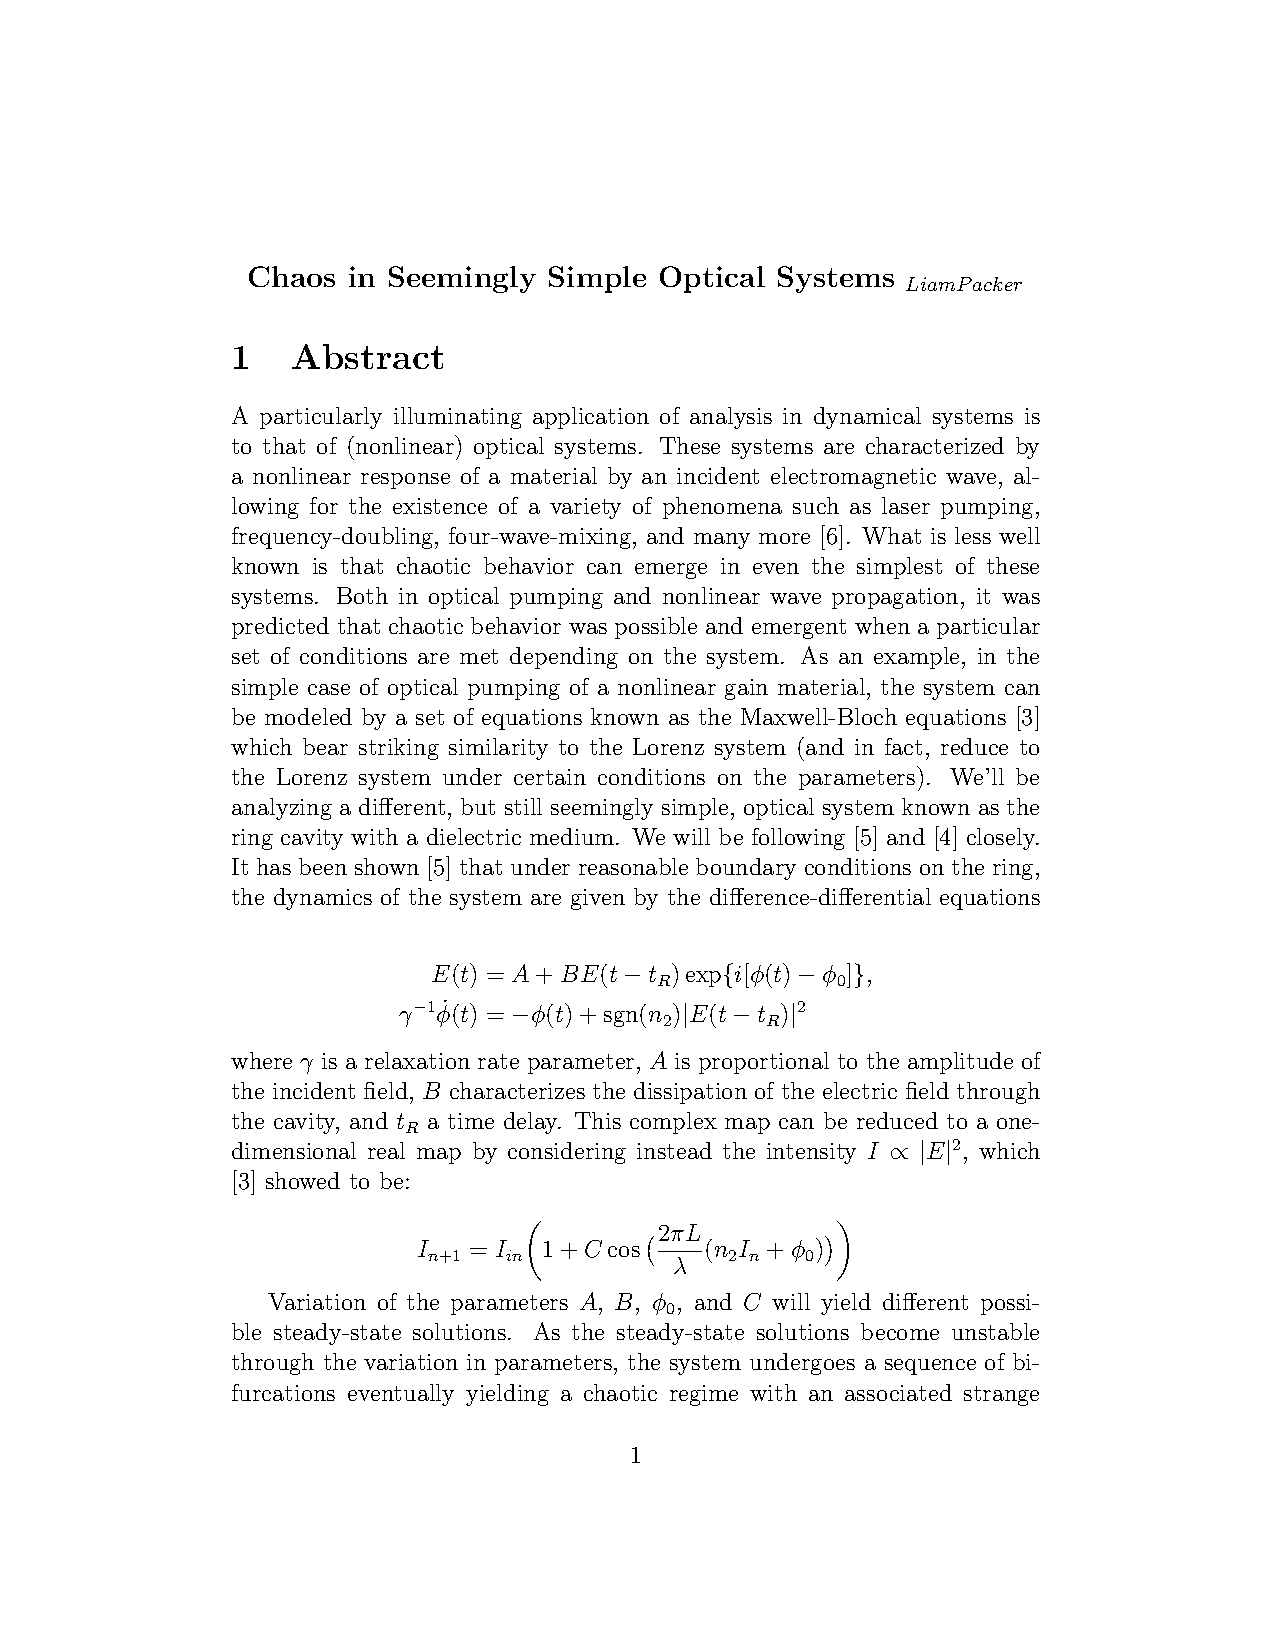
\includegraphics[scale=0.5]{paper.png}}
\caption[]{\label{fig:paper-comp}}
\end{figure}

\begin{figure}[htbp]
\centerline{\includegraphics[scale=0.5]{5.0_2.0_0.4_1_minchaos.png} \includegraphics[scale=0.5]{5.0_2.0_0.4_1_minchaos_zoom.png}}
\centerline{\includegraphics[scale=0.5]{2.0_0.4_1_correlation.png}}
\caption[]{\label{fig:min-chaos}}
\end{figure}

\begin{figure}[htbp]
\centerline{\includegraphics[scale=0.5]{5.0_3.9_0.4_1_paper.png.png} \includegraphics[scale=0.5]{5.0_3.9_0.4_1_paper.png_zoom.png}}
\centerline{\includegraphics[scale=0.5]{3.9_0.4_1_correlation.png}}
\caption[]{\label{fig:paper-chaos} }
\end{figure}

\begin{figure}[htbp]
\centerline{\includegraphics[scale=0.5]{5.0_10.0_0.4_1_paper.png.png} \includegraphics[scale=0.5]{5.0_10.0_0.4_1_paper.png_zoom.png}}
\centerline{\includegraphics[scale=0.5]{10.0_0.4_1_correlation.png}}
\caption[]{\label{fig:max-chaos}}
\end{figure}


\section*{Conclusions}
We started by introducing a simple nonlinear effect in a dielectric medium in the ring
resonator system. From this, clear chaos emerges at a high-intensity input field due to the
system reducing to an iterated map in the adiabatic case $\gamma t_R \to infty$, which
allowed an analysis in either a complex iterated map of the field amplitude \cite{ikeda_optical_1980} or a
real-valued map of the intensity \cite{harrison_chaos_1986}. The results are visually
different but qualitatively similar: chaotic motion. In the case of the complex map, the
result was a fractal of dimension $\approx 1.41$ and in the case of the real map, an orbit
diagram with important qualitative differences from the usual logistic and unmiodal maps.

\bibliographystyle{plain}
\bibliography{refs}
\end{document}

%%% Local Variables:
%%% mode: latex
%%% TeX-master: t
%%% End:
